\chapter{Modelling}

\section{Mass determination of Omega Centauri}

We used various techniques for the determination of the dynamic and stellar mass of NGC5139 that we use to model the mass more accurately. 

\subsection{Stellar Population Synthesis with Starlight}

The stellar mass content of Globular Clusters and Galaxies can be studied through the determination of the stellar populations inside those systems since we have clear knowledge about their photometric properties. If we have information about the amount of stars of a given type inside a stellar system, we can infer how much of the system's mass is given by these populations of stars. 

The determination of the stellar populations can be done using STARLIGHT, which is a Fortran-based program that fits an observed integrated spectrum (Omega Centauri in our case) with a model spectrum which is the sum of $N_{*}$ spectral components from a pre-defined and pre-processed set of base spectra. The program does as many iterations as the user decides to sum up the different template spectra until a good fitting of the spectral lines has been made to the observed spectrum. 

The output of the program after the execution contains the created spectrum (wavelength and intensity) and the approximate percentage of each of the stellar population inside the stellar system. Since the stellar populations are well documented the output will also contain the metallicity of each of them so that further analysis can be made upon STARLIGHT's results.

First, one must prepare the observed spectrum before running STARLIGHT, the spectrum has to be wavelength and flux calibrated, taking into account the bad-pixel removal. Very importantly in the context of mass analysis, the spectrum has to be extinction corrected so that the units of flux relate properly to the units if the templates in STARLIGHT.     

The extinction correction for our observed spectrum is given by

\begin{equation}
f_{obs}(\lambda)=f_{int}(\lambda)10^{-0.4A_{\lambda}}
\end{equation}

Where $A_{\lambda}=0.213$ in the I filter around $8000 \textrm{\AA}$, around the wavelength range of our spectrum. 

On our case, we have to multiply by a factor of 1.216746 the intensity of the spectrum for the flux calibration to be made. After we apply the extinction correction to the spectrum, it is now ready to be processed with STARLIGHT as we can see in the following figure:

\begin{figure}[H]
\centering
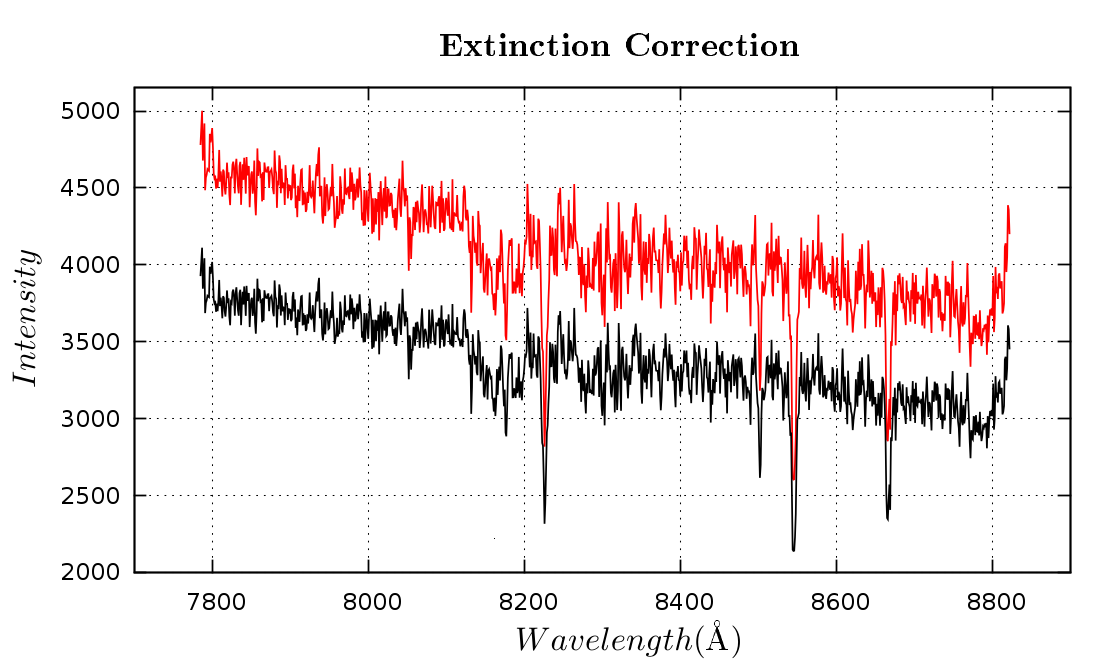
\includegraphics[width=10cm]{images/extinction.png}
\caption[Extinction Correction]{This figure shows an integrated spectrum of the central region of Omega Centauri before and after the extinction correction is applied. The black line has the original flux values and the black line has the corrected flux, that is, the flux that would be observed if there wasn't any interstellar medium that obscures the light coming from the object.}
\end{figure}

Starlight does the stellar population synthesis 

$Mcor_{tot} = 3.29446 \times 10^{7}$

Yields a stellar mass of $M_{*}=243.462M_{\odot}$


\subsection{Modified Hernquist Model}

\subsection{Color-Magnitude diagrams}

